\chapter{Durchführung}
\label{ch:durchfuerung}

\section{Versuchsaufbau}

Der gesamte Versuch wurde auf einer optischen Bank durchgeführt, auf der Lampe, Kondensor, Linsenhalter, Filter, Blenden und Schirme in definierten Abständen montiert werden konnten. Die Justierung erfolgte jeweils so, dass die optische Achse aller Komponenten übereinstimmte. Als Lichtquelle diente eine Halogenlampe mit einstellbarem Kondensor. Zur Reduktion von Farbfehlern wurden Rot-, Blau- und Grünfilter eingesetzt.

\section{Messverfahren}

\subsection{Bestimmung der Parameter der achromatischen Linse}

Zunächst wurde die achromatisch korrigierte Linse (Achromat) zwischen Lampe und Schirm positioniert. Der Gegenstand (Testdia) wurde so ausgerichtet, dass ein scharfes Bild auf dem Schirm erschien. Für verschiedene Gegenstandsweiten $g$ wurden die zugehörigen Bildweiten $b$ bestimmt. In jedem Fall wurde vermerkt, ob das Bild reell oder virtuell und ob es aufrecht oder umgekehrt erschien. Aus den Messwerten lässt sich über \hyperref[eq:linsengleichung]{Gleichung \ref*{eq:linsengleichung}} die Brennweite bestimmen.

\subsection{Brennweitenmessung der bikonvexen Linse nach Bessel}

Zur Bestimmung der Brennweite der bikonvexen Linse $L_1$ wurde das Bessel-Verfahren angewendet. Der Abstand zwischen Gegenstand und Schirm wurde zu $L \approx 5f$ eingestellt. Anschließend wurde die Linse zwischen beiden Positionen verschoben, bis zwei Linsenstellungen mit scharfer Abbildung gefunden wurden. Aus dem Abstand $d$ dieser Positionen ergab sich die Brennweite nach \hyperref[eq:bessel]{Gleichung \ref*{eq:bessel}}. Zur Erhöhung der Genauigkeit wurde der Messvorgang mehrfach wiederholt.

\subsection{Untersuchung der chromatischen und sphärischen Aberration}

Die Messung der Brennweite wurde mit einem Rot- und einem Blaufilter wiederholt, um die chromatische Aberration zu untersuchen. Zusätzlich wurde die Linse einmal mit einer Lochblende und einmal mit einer Ringblende betrieben, um den Einfluss der sphärischen Aberration auf die Brennweite zu beobachten. Veränderungen des Abstandes $d$ zwischen den Bessel-Positionen deuten auf Unterschiede in der effektiven Brennweite hin.

\subsection{Aufbau und Untersuchung eines Mikroskops}

Für die Untersuchung des Mikroskops wurde eine Kombination aus Objektiv- und Okularlinse auf der optischen Bank aufgebaut. Als Objekt diente ein Kreuzgitter-Dia, das hinter einer Lampe mit Grünfilter positioniert wurde. Das Zwischenbild wurde in einem definierten Abstand zur Objektivlinse auf einem Schirm abgebildet, der eine Millimeterskala trug. Hinter dem Zwischenbild wurde das Okular in seiner Brennweite positioniert, sodass das Auge auf unendlich akkommodierte.

Die Vergrößerung wurde aus der Gitterstruktur des Zwischenbilds bestimmt. Anschließend wurde der einstellbare Spalt schrittweise verengt, bis die vertikalen Strukturen des Gitters gerade nicht mehr aufgelöst werden konnten. Aus der Spaltbreite und dem Abstand zum Objekt wurde der Öffnungswinkel berechnet, aus dem sich mit \hyperref[eq:auflösung]{Gleichung \ref*{eq:auflösung}} das Auflösungsvermögen ergab. Der Versuch wurde mit rotem und blauem Licht wiederholt, um den Einfluss der Wellenlänge auf die Auflösung zu überprüfen.

\begin{figure}[b!]
    \centering
    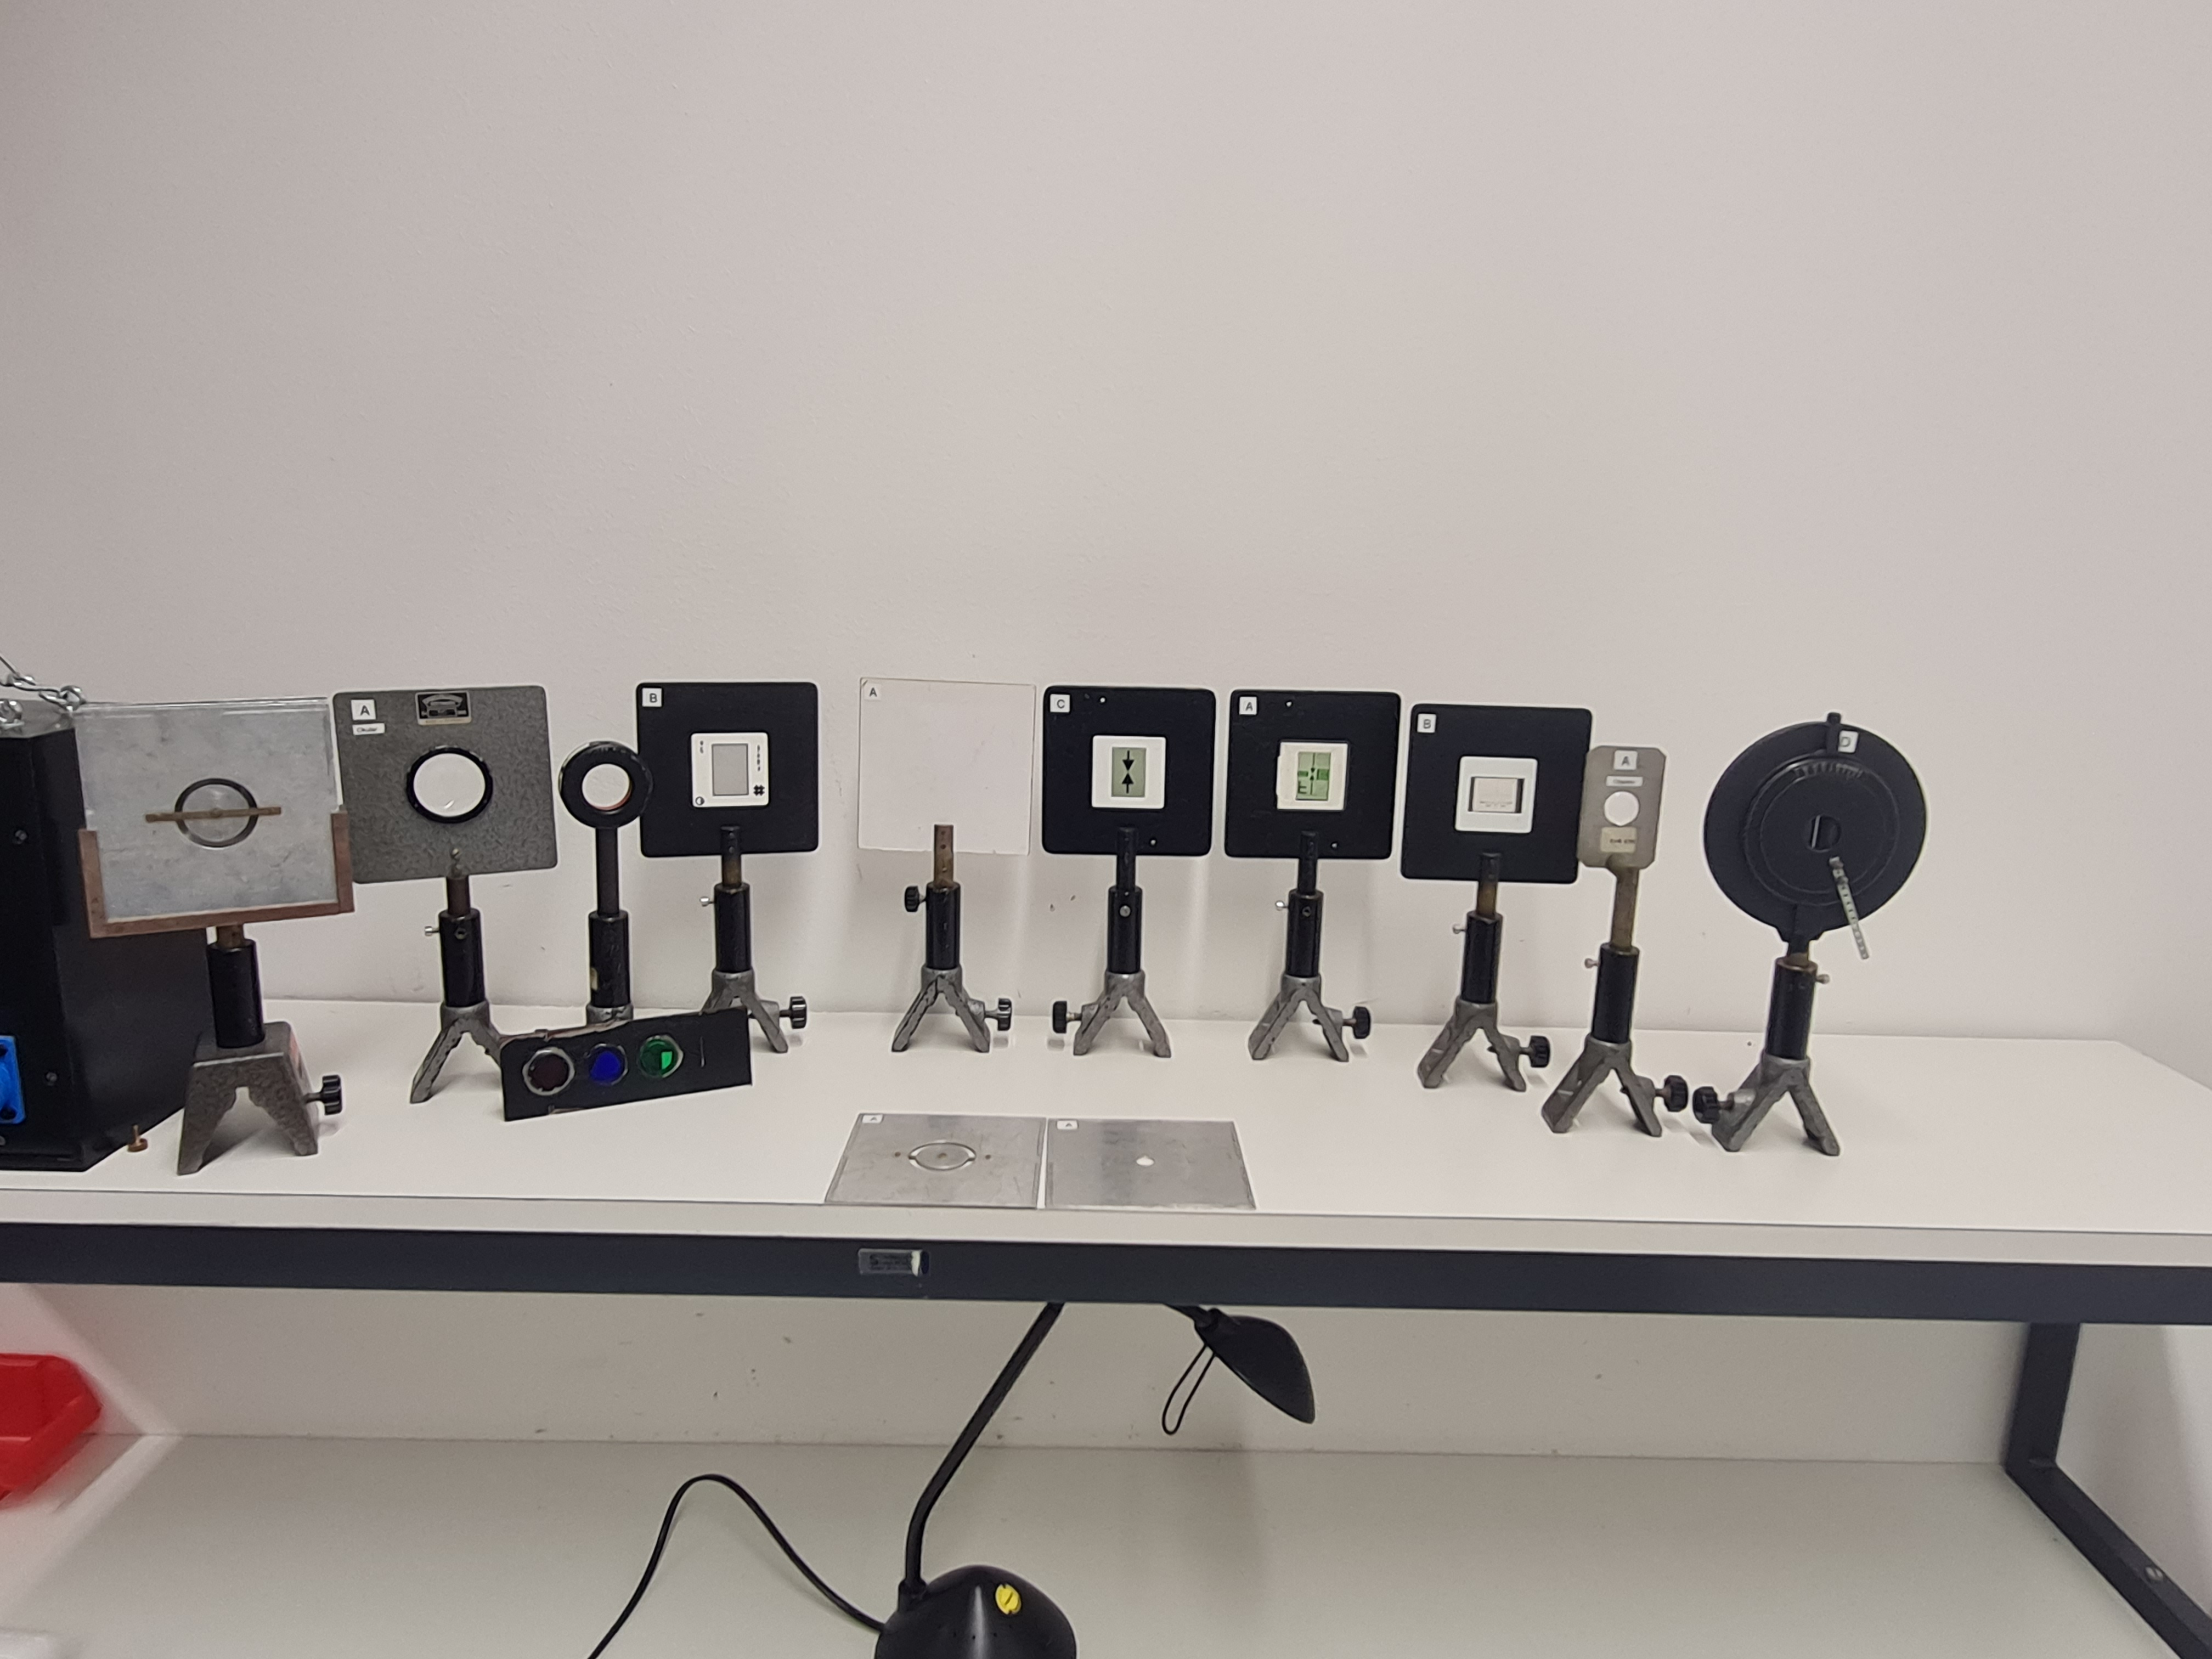
\includegraphics[width=\textwidth]{img/31/Versuchsbestandteile.jpg}
    \caption{Versuchsbestandteile}
\end{figure}

\onecolumn
\begin{figure}
    \centering
    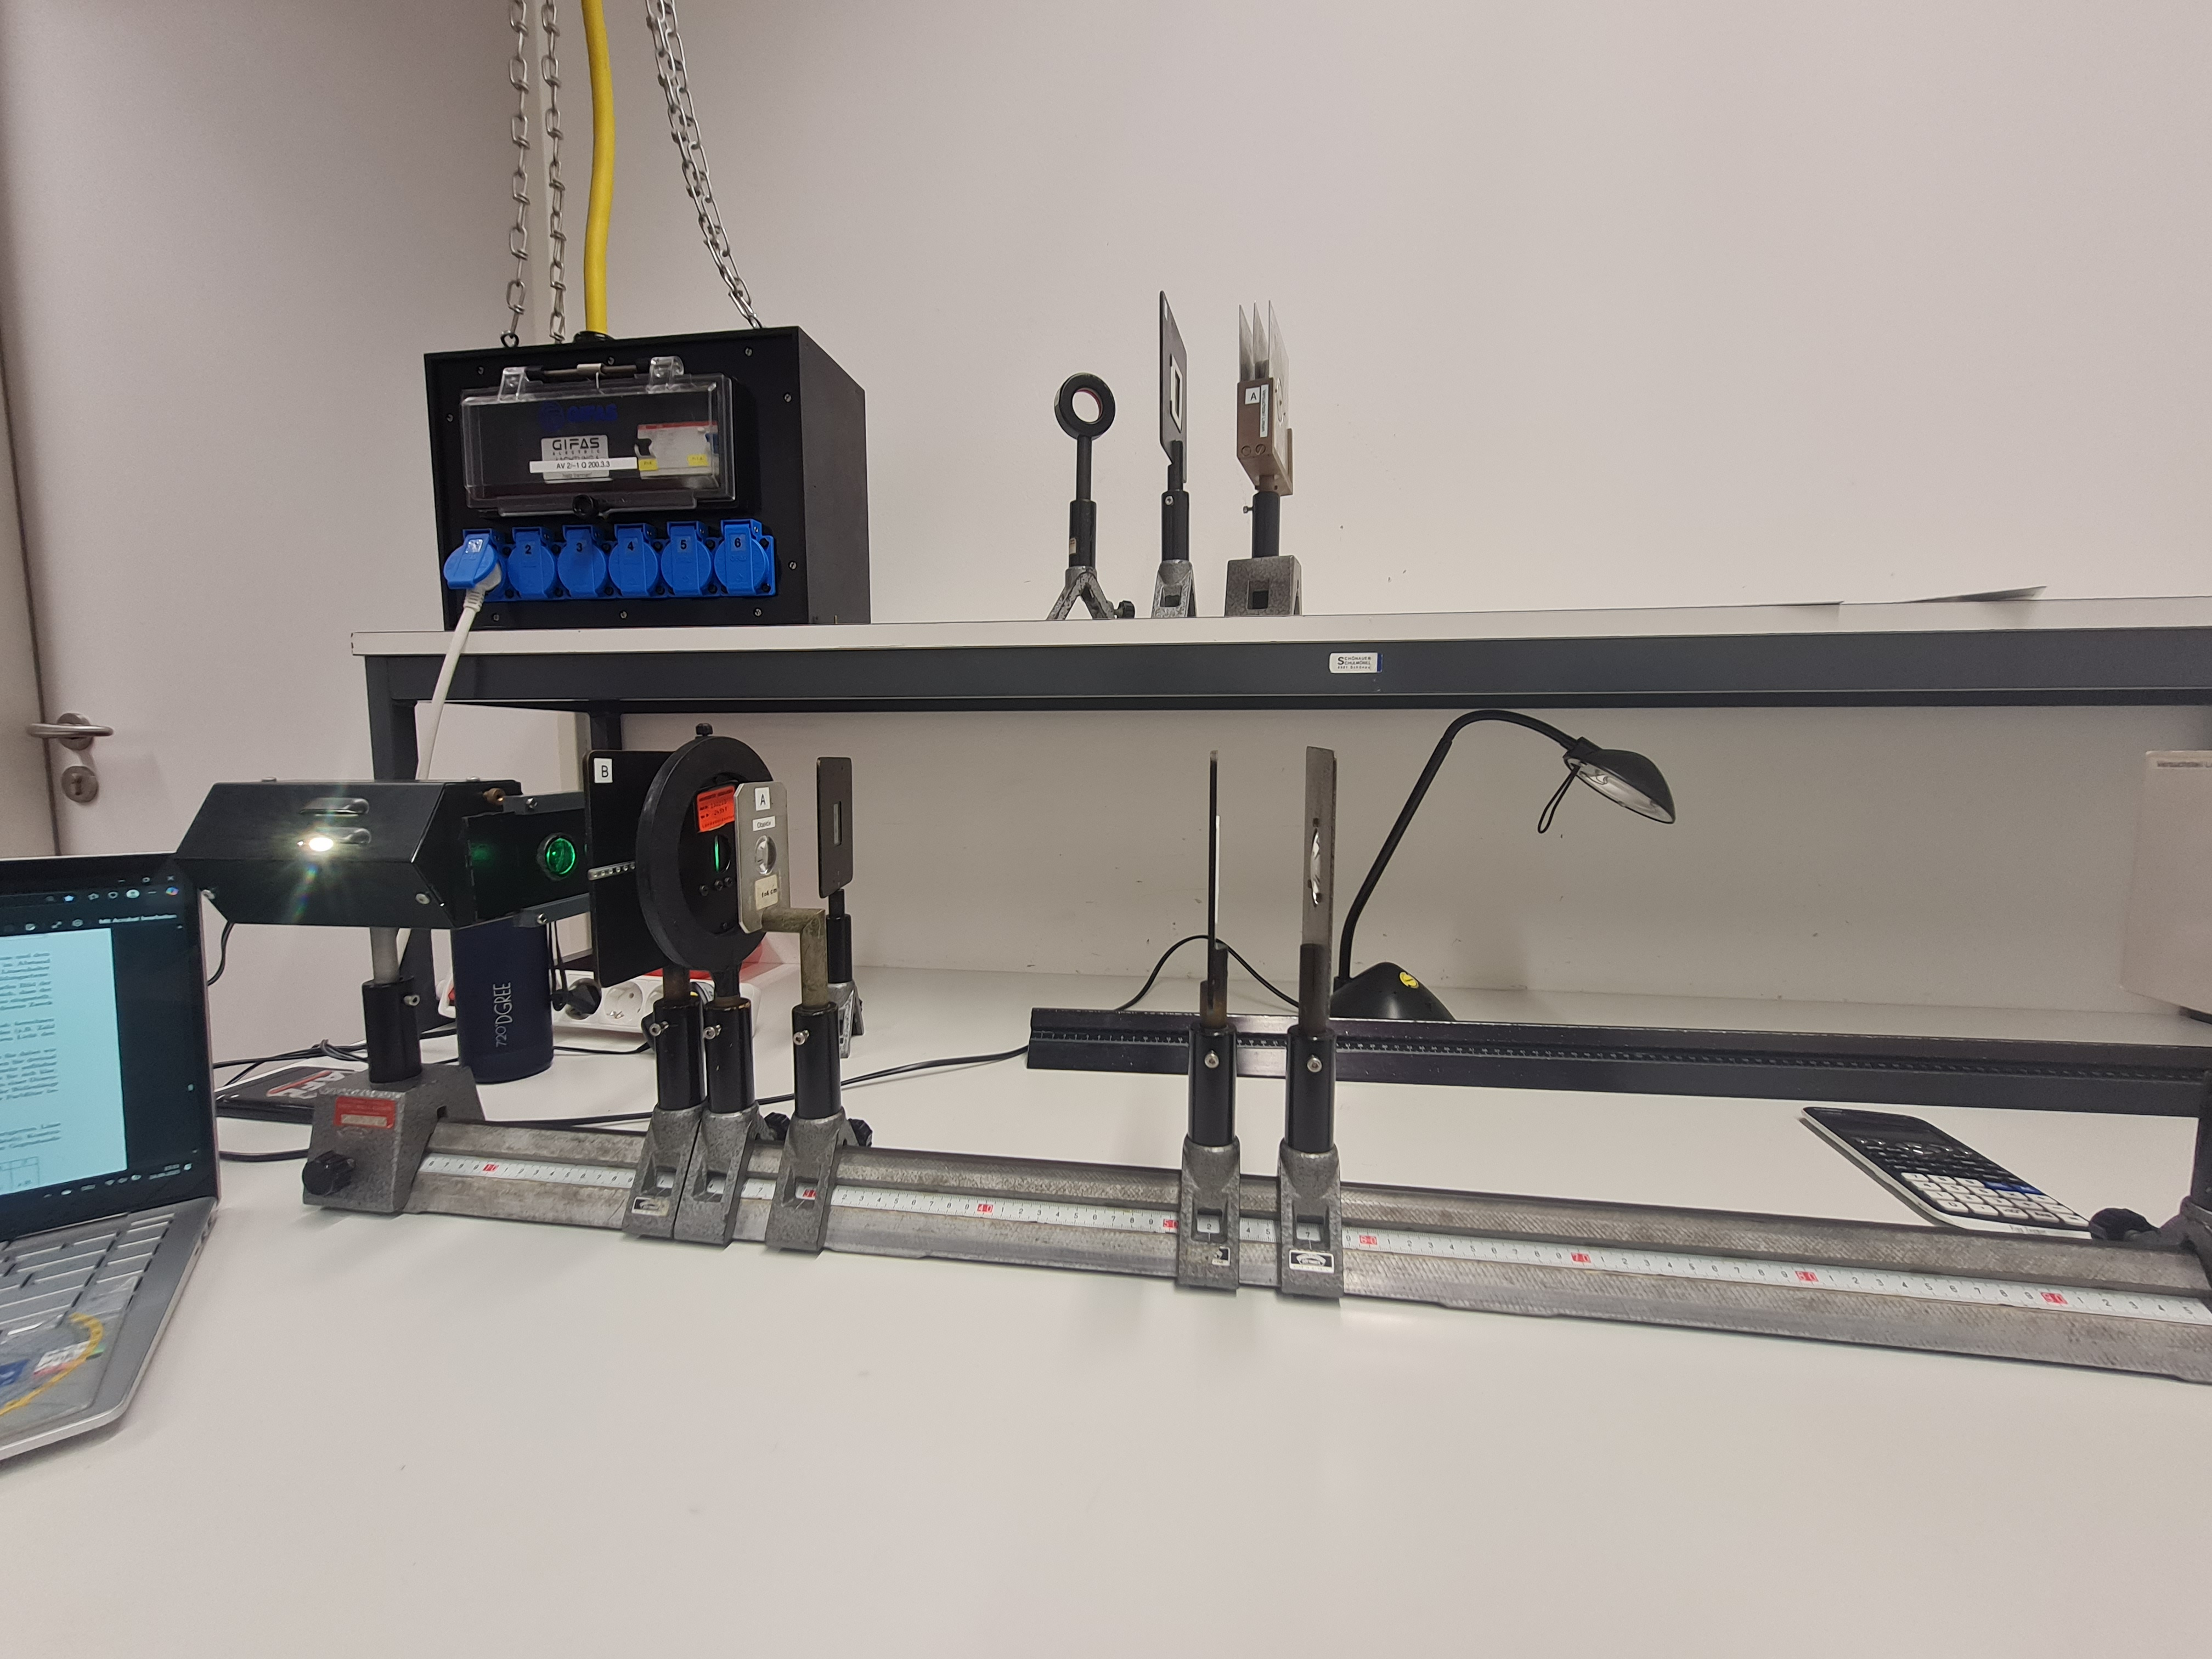
\includegraphics[width=\textwidth]{img/31/A2.jpg}
    \caption{Versuchsaufbau Aufgabe Gitter}
\end{figure}

\begin{figure}
    \centering
    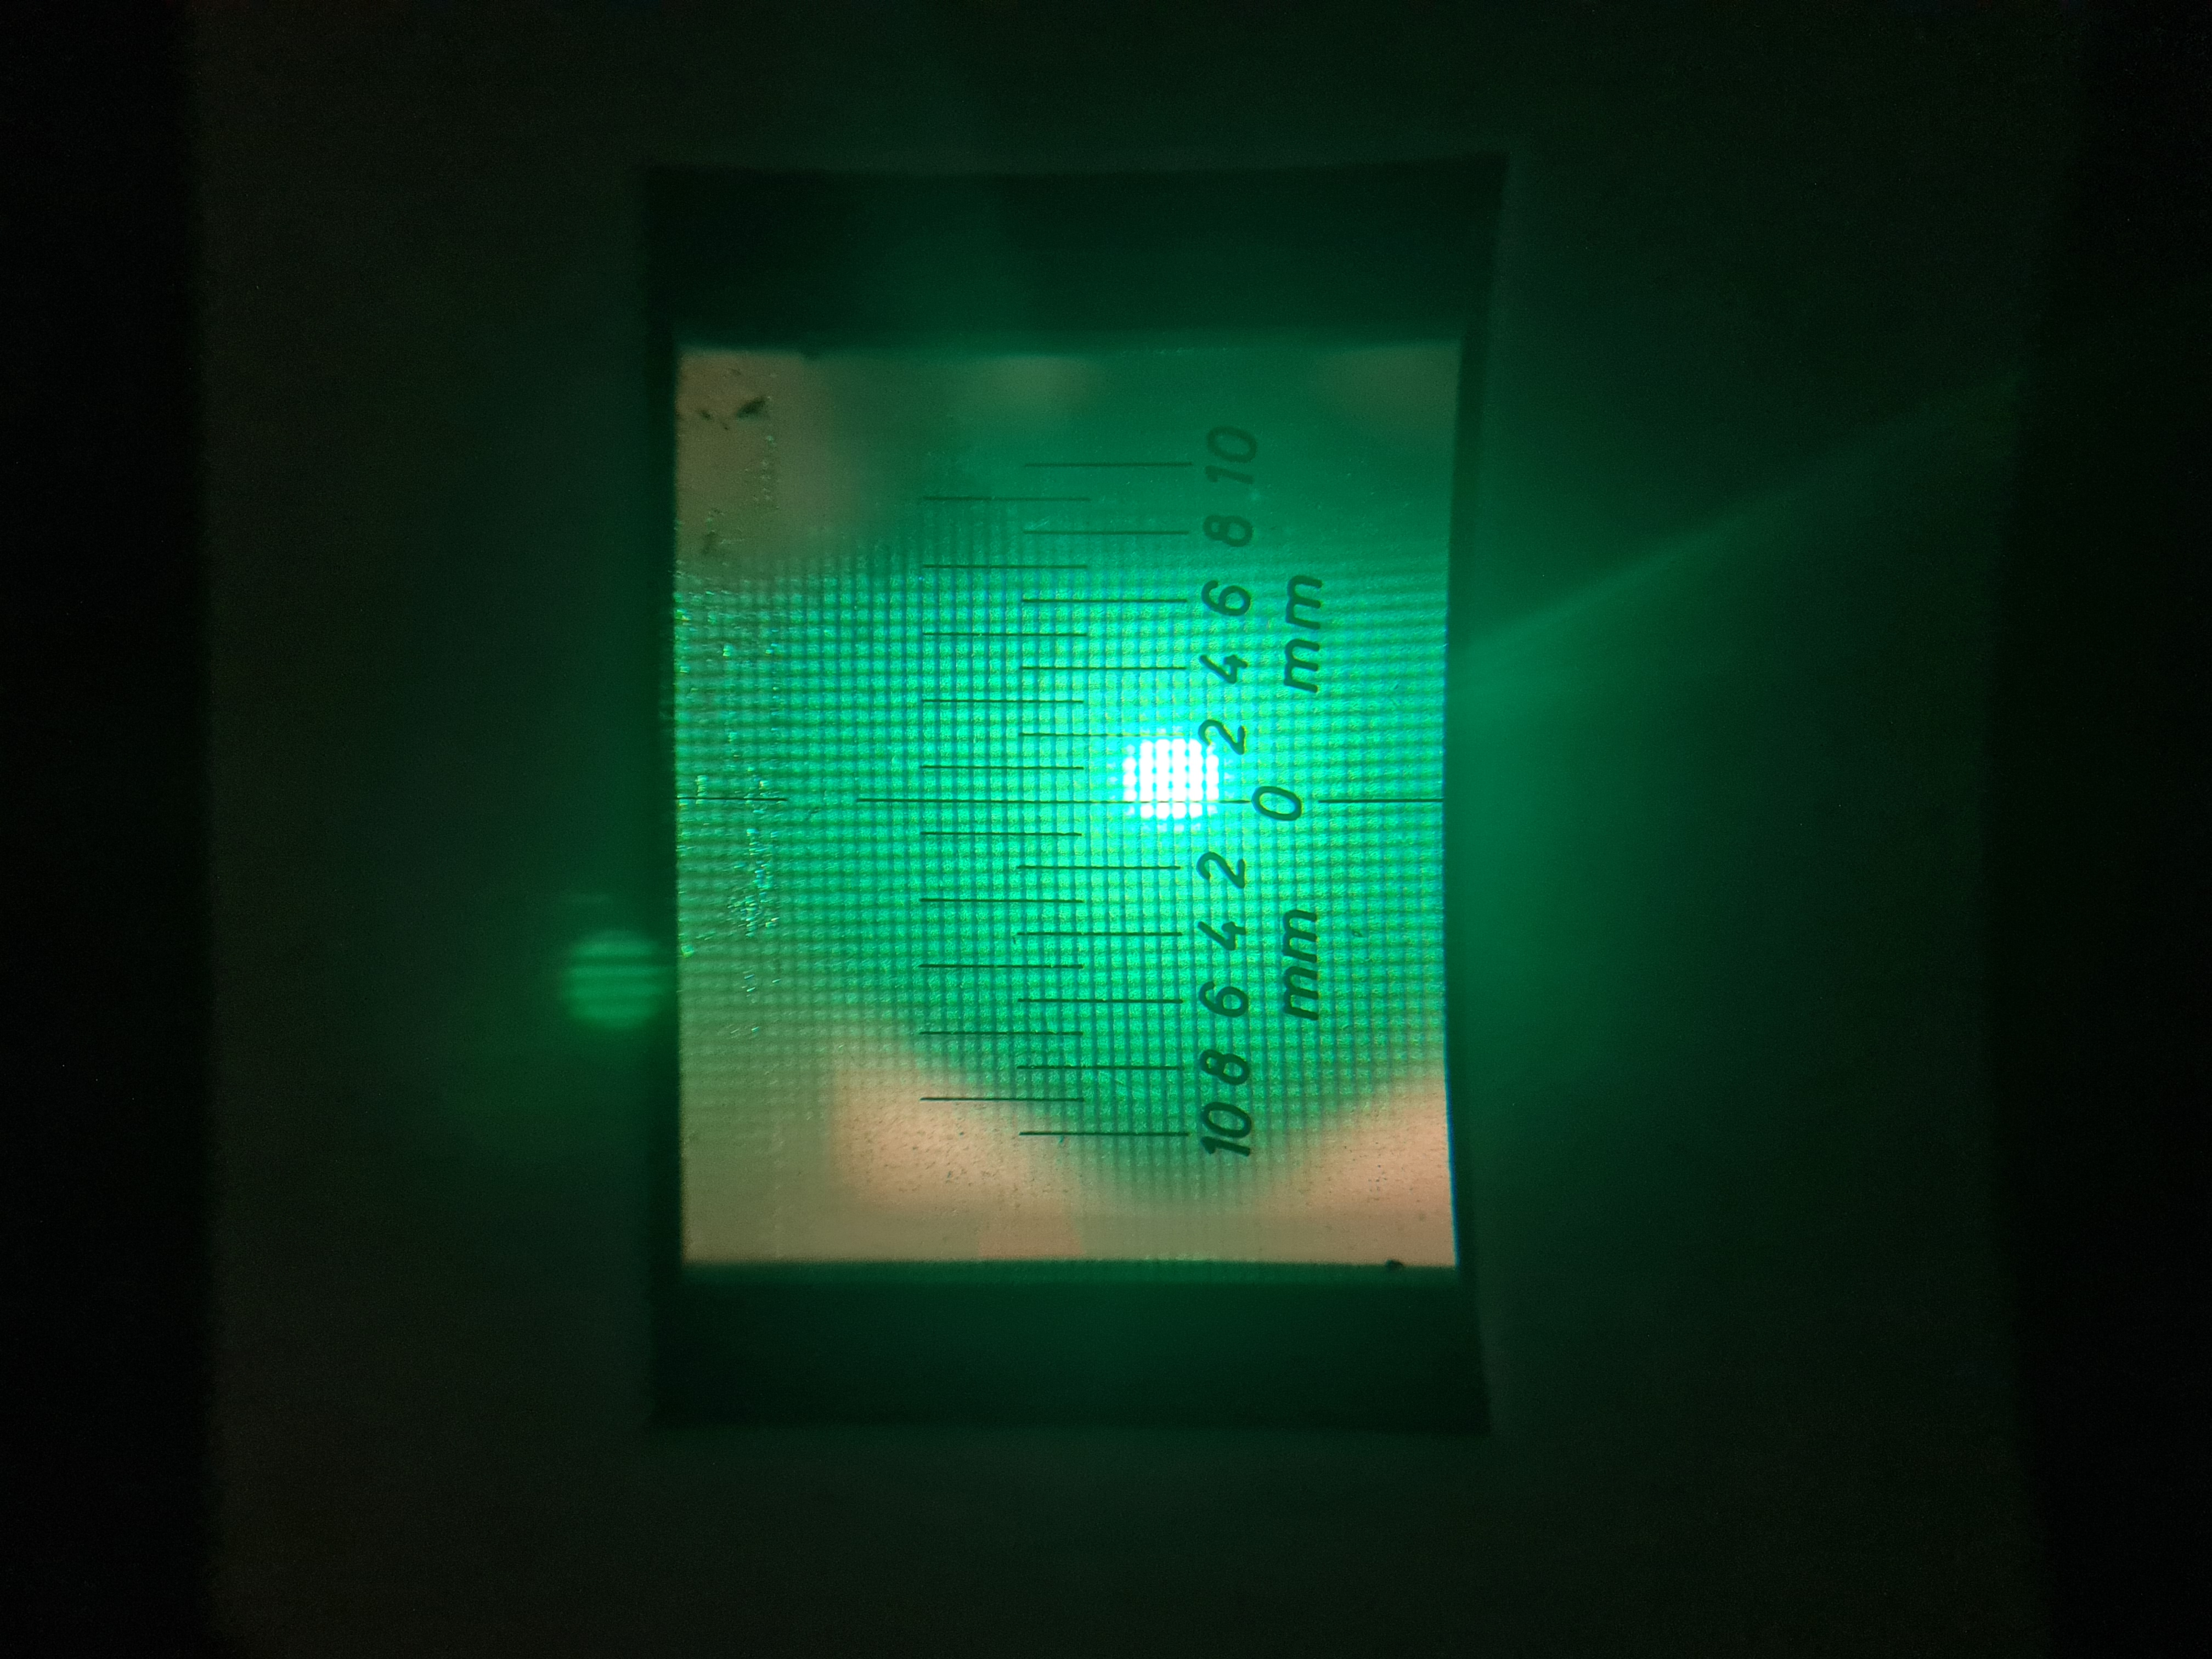
\includegraphics[width=\textwidth]{img/31/Gitter.jpg}
    \caption{Blich durch das Mikroskop auf das Gitter}
\end{figure}

\twocolumn